\documentclass[]{article}

\usepackage{algorithmic}
\usepackage{algorithm}
\usepackage{amsmath}
\usepackage{amssymb}
\usepackage{amsthm}
\usepackage{etoolbox}
\usepackage{hyperref}
\usepackage{ifdraft}
\usepackage{listings}
\usepackage{mathtools}
\usepackage{pgfplots}
\usepackage{siunitx}
\usepackage{subcaption}
\usepackage[obeyFinal]{todonotes}


%math typeseting
\newcommand{\mat}[1]{\mathbf{#1}}
\DeclarePairedDelimiter\ceil{\lceil}{\rceil}
\DeclarePairedDelimiter\floor{\lfloor}{\rfloor}

\pgfplotsset{compat=1.16}

%number the bib as a section
\patchcmd{\thebibliography}{\section*}{\section}{}{}


%
%note TODO notes are hidden in draft mode to improve compile times
\newcommand{\review}[1]{\ifdraft{}{\todo[linecolor=yellow,backgroundcolor=yellow!25,bordercolor=yellow]{REVIEW: #1}}}
\newcommand{\change}[1]{\ifdraft{}{\todo[linecolor=red,backgroundcolor=red!25,bordercolor=red]{TODO: #1}}}
\newcommand{\info}[1]{\ifdraft{}{\todo[linecolor=blue,backgroundcolor=blue!25,bordercolor=blue]{INFO: #1}}}

\begin{document}

%Example environment
\theoremstyle{definition}
\newtheorem{example}{Example}

\begin{titlepage}
	\begin{center}
		\vspace*{1cm} 
		\LARGE{\textbf{\input{title.txt}}}
		
		\vspace{0.5cm}
		\Large{An All-College Thesis}
		
		\vspace{2cm}
		\Large{College of Saint Benedict/Saint John's University}
		
		\vspace{2cm}
		
		\large{by Neil Lindquist}
		
		\large{April 2018}
		
	\end{center}
\end{titlepage}

% textidote: ignore begin
%Signature page
\begin{flushleft}
	\large{\textbf{Project Title:} \input{title.txt}}\\
	Approved by:\\
	\vspace{1cm}
	\hrulefill \\
	\large{Mike Heroux}\\
	\small{Scientist in Residence}\\
	\vspace{1.5cm}
	\hrulefill \\
	\large{Robert Hesse}\\
	\small{Associate Professor of Math}\\
	\vspace{1.5cm}
	\hrulefill \\
	\large{Jeremy Iverson}\\
	\small{Assistant Professor of Computer Science}\\
	\vspace{1.5cm}
	\hrulefill \\
	\large{Bret Benesh}\\
	\small{Chair, Department of Mathematics}\\
	\vspace{1.5cm}
	\hrulefill \\
	\large{Imad Rahal}\\
	\small{Chair, Department of Computer Science}\\
	\vspace{1.5cm}
	\hrulefill \\
	\small{Director, All College Thesis Program}\\
\end{flushleft}
% textidote: ignore end

\clearpage

\vspace*{\fill}
\begin{abstract}
	Solving large, sparse systems of linear equations plays an important role in certain scientific computations.
	However, these solvers usually spend most of their time fetching data from main memory.
	To improve the performance of these solvers, this work explores using data compression to reduce memory accesses.
	Some compression methods were found that improve the performance of the solver and problem found in the HPCG benchmark by up to 85\%.
	\change{This seems too short}
\end{abstract}
\vspace*{\fill}

\clearpage

\tableofcontents

\clearpage

\section{Introduction}
Solving large, sparse linear systems of equations plays a vital role in certain scientific computations.
For example, the finite element method solves a system of linear equations to approximate the solution to certain partial differential equations~\cite{Saad:2003:IterativeMethods}.
These problems can be large, with easily millions of variables or more~\cite{Davis:2011:FloridaMatrixCollection}.
So, solving these problems efficiently requires a fast linear solver.

Iterative solvers are often used to solve these large, sparse systems.
These solvers take an initial guess then improve it until it is within some tolerance~\cite{Saad:2003:IterativeMethods}.
On modern computers, these solvers often spend most of their time fetching data from main memory to the processor where the actual computation is done~\cite{Lawlor:2013:compression}.
This work tries to improve the performance of iterative solvers by compressing the data to reduce the time spent accessing main memory.

To avoid implementing an entire sparse linear solver, the High Performance Conjugate Gradient (HPCG) benchmark was used as the initial codebase for the project~\cite{Dongarra:2015:HPCG}.
The HPCG benchmark is designed to measure the performance of computing systems when processing sparse solvers and does so by solving one such test problem.
In addition, as a benchmark, HPCG has built in measurements of elapsed time, solver iterations and the number of floating point operations that needed to be computed.
These factors all make the HPCG codebase a natural starting point for developing improvements to sparse, iterative linear solvers.

There are three main data structures that were experimented with in this project: the vector values, the matrix values, and the matrix indices.
For each of these data structures, compression methods were found that were able to fulfill the requirements on read and write access.
Additionally, two models were constructed to estimate the minimum performance a compression method would need to outperform the baseline.
Both models indicated that vector values must be decoded with only a few instructions, but that decoding the matrix values has a much larger, but still limited, window for improvement.
In the actual tests, a couple of configurations were found to be able to outperform the baseline implementation, with an increase in performance of up to 84\%.

\subsection{Previous Work}
First, this work draws heavily on existing data compression methods.
Some of the algorithms used were designed with scientific computations in mind, such as ZFP and SZ compression~\cite{Lindstrom:2014:zfp,Di:2016:SZ}.
Other algorithms are more general purpose, such as Huffman and Elias Codings~\cite{Huffman:1952:coding,Elias:1975:codeword}.
Section~\ref{sec:bg-comp} goes into detail on what compression methods were used and how they work.

Much work has been done on various aspects of utilizing single precision floating point numbers while retaining the accuracy of double precision numbers in iterative linear solvers.
One approach, which this work draws inspiration from, is to apply the preconditioner using single precision, while otherwise using double precision, which result in similar accuracy unless the matrix is poorly conditioned~\cite{Buttari:2008:mixedPrec, Hogg:2010:multiplePasses}.
This strategy of mixing floating point precision for various parts of the solver algorithm leads to the use of making certain vectors single precision, as described in Section~\ref{sec:bg-comp-floatPrec}.

Another effort at compressing large, sparse Linear Systems is Compressed Column Index (CCI) format to store matrices~\cite{Lawlor:2013:compression}.
This format is based on Compressed Sparse Row (CSR) matrix format except uses compression to reduce the size of the matrix indices.
The index compression used by CCI is described in Section~\ref{sec:bg-comp-opcode} and tested in this project.
This project generalizes the ideas of CCI matrices, both by compressing additional data structures and using additional compression methods.
However, only a single matrix is tested for this project, as opposed to the suite of matrices used to look at the performance of CCI matrices.

\subsection{Mathematics of Conjugate Gradient}
Conjugate Gradient is the iterative solver used by HPCG~\cite{Dongarra:2015:HPCG}.
Symmetric, positive definite matrices will guarantee the converge of Conjugate Gradient to the correct solution within \(n\) iterations, where \(n\) is the rows of the matrix, when using exact algebra~\cite{Saad:2003:IterativeMethods}.
More importantly, Conjugate Gradient can be used as in iterative method, providing a solution, \(\vec{x}\), where \(\left\|\mat{A}\vec{x}-\vec{b}\right\|\) is within some tolerance, after significantly fewer than \(n\) iterations, allowing it to find solutions to problems where computing \(n\) iterations is infeasible~\cite{Shewchuk:1994:IntroToCG}.
As an iterative method, Conjugate Gradient forms update directions from Krylov subspaces of the form \(\mathcal{K}_n(\vec{r}_0, \mat{A})=\text{span}(\vec{r}_0, \mat{A}\vec{r}_0, \mat{A}^2\vec{r}_0, \dots, \mat{A}^n\vec{r}_0)\), where \(\vec{r}=\vec{b}-\mat{A}\vec{x}_0\).

%Steepest Decent
To understand the Conjugate Gradient, first consider the quadratic form of \(\mat{A}\vec{x} = \vec{b}\).
The quadratic form is a function \(f:\mathbb{R}^n\to\mathbb{R}\) where
\begin{equation}
\label{eq:cg-quad-form}
	f(\vec{x}) = \tfrac{1}{2}\vec{x}^T\mat{A}\vec{x} - \vec{b}\cdot\vec{x} + c
\end{equation}
for some \(c\in\mathbb{R}\).
Note that
\[
	\nabla f\left(\vec{x}\right) = \tfrac{1}{2}\left(\mat{A}+\mat{A}^T\right)\vec{x}-\vec{b}
\]
Then, when \(\mat{A}\) is symmetric,
\begin{equation*}
	\nabla f(\vec{x}) = \mat{A}\vec{x} - \vec{b}
\end{equation*}
So, the solution to \(\mat{A}\vec{x} = \vec{b}\) is the sole critical point of \(f\)~\cite{Nearing:2010:toolsForPhysics}.
Since \(\mat{A}\) is the Hessian matrix of \(f\) at the point, if \(\mat{A}\) is positive definite, then that critical point is a minimum.
Thus, if \(\mat{A}\) is a symmetric, positive definite matrix, then the minimum of \(f\) is the solution to \(\mat{A}\vec{x} = \vec{b}\)~\cite{Shewchuk:1994:IntroToCG}.

The method of Steepest Decent is useful for understanding Conjugate Gradient, because they both use a similar approach to minimize Equation~\ref{eq:cg-quad-form}, and thus solve \(\mat{A}\vec{x}=\vec{b}\).
This shared approach is to take an initial \(\vec{x}_0\) and move downwards in the steepest direction, within certain constraints, of the surface defined by Equation~\ref{eq:cg-quad-form}~\cite{Nearing:2010:toolsForPhysics}.
Because the gradient at a point is the direction of maximal increase, \(\vec{x}\) should be moved in the opposite direction of the gradient.
Thus, to compute the next value of \(\vec{x}\), use
\begin{equation}
\label{eq:cg-xUpdate}
	\vec{x}_{i+1} = \vec{x}_i + \alpha_i \vec{r}_i
\end{equation}
for some \(\alpha_i > 0\) and where \(\vec{r}_i = -\nabla f\left(\vec{x}_i\right) = \vec{b} - \mat{A}\vec{x}_i\) is the residual of \(\vec{x}_i\).
Since \(\mat{A}\vec{x} = \vec{b}\) is the only critical point and a minimum of the quadratic function, \(f\), the ideal value of \(\alpha_i\) is the one that minimizes \(f\left(\vec{x}_{i+1}\right)\).
Thus, choose \(\alpha_i\) such that
\begin{align*}
	0
	&= \tfrac{\mathrm{d}}{\mathrm{d} \alpha_i} f\left(\vec{x}_{i+1}\right) \\
	&= \tfrac{\mathrm{d}}{\mathrm{d} \alpha_i} f\left(\vec{x}_i + \alpha \vec{r}_i\right) \\
%
	\alpha_i
	&= \frac{\vec{r}_i\cdot \vec{r}_i}{\vec{r}_i\cdot\mat{A}\vec{r}_i}.
\end{align*}
Note that by using Equation~\ref{eq:cg-xUpdate}, we can derive
\begin{equation}
\label{eq:CG-improvedResidual}
	\vec{r}_{i+1} = \vec{r}_i - \alpha\mat{A}\vec{r}_i.
\end{equation}
Because \(\mat{A}\vec{r}_i\) is already computed to find \(\alpha_i\), using Equation~\ref{eq:CG-improvedResidual} to compute the residual results in one less matrix-vector product per iteration.
Algorithm~\ref{alg:bg-cg-alg-steepestDecent} shows the resulting algorithm.
\begin{algorithm}[tb]
	\begin{algorithmic}
		\STATE \(\vec{r}_0 \gets \vec{b} - \mat{A}\vec{x}_0\)
		\FOR{\(i = 0, 1, \dots\) \textbf{until} \(\left\|\vec{r}_i\right\| \leq \epsilon\)}
			\STATE \(\alpha_i \gets \frac{\vec{r}_i\cdot \vec{r}_i}{\vec{r}_i\cdot\mat{A}\vec{r}_i}\)
			\STATE \(\vec{x}_{i+1} = \vec{x}_i + \alpha_i\vec{r}_i\)
			\STATE \(\vec{r}_{i+1} = \vec{r}_i - \alpha\mat{A}\vec{r}_i\)
		\ENDFOR
	\end{algorithmic}
	
	\caption{Steepest Decent~\cite{Shewchuk:1994:IntroToCG}.}
	\label{alg:bg-cg-alg-steepestDecent}
\end{algorithm}


\begin{example}
\label{ex:CG-SteepestDecent}
%x = (2, 1)
Consider the linear system
\[
	\mat{A} = \begin{bmatrix}
		2 & 1 \\
		1 & 3
	\end{bmatrix},
	\quad
	\vec{b} = \begin{bmatrix}
		5 \\
		5 
	\end{bmatrix}
\]
and use \(c=0\).
Note that the solution is
\[
	\vec{x} = \begin{bmatrix}
		2 \\ 1
	\end{bmatrix}.
\]
When starting at the origin, the iteration of Method of Steepest Decent becomes
\begin{align*}
	 \vec{x}_0 &= \begin{bmatrix}0\\0\end{bmatrix}
	&\vec{r}_0 &= \begin{bmatrix}5\\5\end{bmatrix}
	&\alpha_0  &= 2/7 \\
	%
	 \vec{x}_1 &= \begin{bmatrix}10/7\\10/7\end{bmatrix}
	&\vec{r}_1 &= \begin{bmatrix}5/7\\-5/7\end{bmatrix}
	&\alpha_1  &= 2/3 \\
	%
	 \vec{x}_2 &= \begin{bmatrix}40/21\\20/21\end{bmatrix}
	&\vec{r}_2 &= \begin{bmatrix}5/21\\5/21\end{bmatrix}
	&\alpha_2  &= 2/7 \\
	%
	 \vec{x}_3 &= \begin{bmatrix}290/147\\50/49\end{bmatrix}
	&\vec{r}_3 &= \begin{bmatrix}5/147\\-5/147\end{bmatrix}
	&\alpha_3  &= 2/3 \\
	%
	&\vdots &&\vdots &&\vdots
\end{align*}
The \(\vec{x}_i\)s are plotted with a contour graph of the quadratic form in Figure~\ref{fig:CG-steepestDecentExample-Iterations}. \qed
\begin{figure}
	\centering
	\ifdraft{}{
		\begin{tikzpicture}
			\begin{axis} [
				xlabel=\(x_1\),
				ylabel=\(x_2\),
				view={0}{90},
			]
				\addplot3 [
					domain=0:4,
					domain y=0:4,
					samples=50,
					samples y=50,
					contour gnuplot={
						levels={-7, -5, -3, -1, 1, 3, 5, 7, 9, 11, 13},
						labels=false,
						draw color=black,
						handler/.style=smooth
					},
				] {.5*(2*x^2 + 2*x*y + 3*y^2) - 5*x - 5*y};
				
				\addplot[black,mark=none] coordinates {(0,0)  (10/7, 10/7)  (40/21, 20/21)  (290/147,50/49) (880/441,440/441) (6170/3087,1030/1029)};
			\end{axis}
		\end{tikzpicture}
	}
	
	\caption{Contour graph of the quadratic function and the first six values of \(\vec{x}\) produced by steepest decent for Example~\ref{ex:CG-SteepestDecent}}
	\label{fig:CG-steepestDecentExample-Iterations}
\end{figure}
\end{example}

%Conjugate Directions
The Conjugate Directions family of linear solvers, of which Conjugate Gradient is a member of, attempts to improve on the number of iterations needed by Steepest Decent.~\cite{Shewchuk:1994:IntroToCG}.
Note that, in Example~\ref{ex:CG-SteepestDecent}, the directions of \(\vec{r}_0\) and \(\vec{r}_2\) are the same and the directions of \(\vec{r}_1\) and \(\vec{r}_3\) are the same.
Thus, the same direction is traversed multiple times.
Additionally, note that the two sets of residual directions are perpendicular to each other.
Conjugate Directions attempts to improve on this, by making the search directions, \(\vec{d}_0, \vec{d}_1, \dots\), \(\mat{A}\)-orthogonal to each other and only moving \(\vec{x}\) once in each search direction.
Two vectors, \(\vec{u}, \vec{v}\), are \(\mat{A}\)-orthogonal, or conjugate, if \(\vec{u}^T\mat{A}\vec{v}=0\).
The requirement for Conjugate Directions is to make \(\vec{e}_{i+1}\) \(\mat{A}\)-orthogonal to \(\vec{d}_i\), where \(\vec{e}_i = \vec{x}_i - \mat{A}^{-1}\vec{b}\) is the error of \(\vec{x}_i\).
The computation of \(\alpha_i\) changes to find the minimal value along \(\vec{d}_i\) instead of \(\vec{r}_i\).
\[
	\alpha_i = \frac{\vec{d}_i^T\vec{r}_i}{\vec{d}_i^T\mat{A}\vec{d}_i}.
\]

%Conjugate Gradient proper
Conjugate Gradient is a form of Conjugate Directions where the residuals are made to be \(\mat{A}\)-orthogonal to each other~\cite{Shewchuk:1994:IntroToCG}.
This is done using the Conjugate Gram-Schmidt Process.
To do this, each search direction, \(\vec{d}_i\) is computed by taking \(\vec{r}_i\) and removing any components that are not \(\mat{A}\)-orthogonal to the previous \(\vec{d}\)'s~\cite{Shewchuk:1994:IntroToCG}.
So, let \(\vec{d}_0 = \vec{r}_0\) and for \(i > 0\) let
\[
	\vec{d}_i = \vec{r}_i + \sum_{k=0}^{i-1} \beta_{(i, k)}\vec{d}_k
\]
with \(\beta_{(i, k)}\) defined for \(i > k\).
Then, solving for \(\beta_{(i, k)}\) gives
\[
	\beta_{(i, k)} = -\frac{\vec{r}_i\cdot\mat{A}\vec{d}_i}{\vec{d}_j\cdot\mat{A}\vec{d}_j}.
\]
Note that each residual is orthogonal to the previous search directions, and thus the previous residuals.
So, it can be shown that \(\vec{r}_{i+1}\) is \(\mat{A}\)-orthogonal to all previous search directions, except \(\vec{d}_i\)~\cite{Shewchuk:1994:IntroToCG}.
Then, \(\beta_{(i, k)} = 0\) for \(i-1 \neq k\).
To simplify notation, let \(\beta_i = \beta_{(i, i-1)}\).
So, each new search direction can then be computed by
\[
	\vec{d}_i = \vec{r}_i + \beta_i\vec{d}_{i-1}.
\]
Algorithm~\ref{alg:bg-cg-alg-cg} shows the final Conjugate Gradient algorithm.

\begin{algorithm}[tb]
	\begin{algorithmic}
		\STATE \(\vec{r}_0 \gets \vec{b} - \mat{A}\vec{x}_0\)
		\STATE \(\vec{d}_0 \gets \vec{r}_0\)
		\FOR{\(i = 0, 1, \dots\) \textbf{until} \(\left\|\vec{r}_i\right\| \leq \epsilon\)}
			\STATE \(\alpha_i \gets \frac{\vec{r}_i\cdot\vec{r}_i}{\vec{d}_i\cdot \mat{A}\vec{d}_i}\)
			
			\STATE \(\vec{x}_{i+1} \gets \vec{x}_i + \alpha_i\vec{d}_i\)
			\STATE \(\vec{r}_{i+1} \gets \vec{r}_i + \alpha_i\mat{A}\vec{d}_i\)
			\STATE \(\beta_{i+1} \gets \frac{\vec{r}_{i+1}\cdot\vec{r}_{i+1}}{\vec{r}_i\cdot\vec{r}_i}\)
			\STATE \(\vec{r}_{i+1} + \beta_{i+1}\vec{d}_i\)
		\ENDFOR
	\end{algorithmic}
	
	\caption{Conjugate Gradient~\cite{Saad:2003:IterativeMethods}.}
	\label{alg:bg-cg-alg-cg}
\end{algorithm}


% 2 1
% 1 3
\begin{example}
\label{ex:CG-CG}
Consider the linear system used in Example~\ref{ex:CG-SteepestDecent} where
\[
	\mat{A} = \begin{bmatrix} 2 & 1 \\ 1 & 3 \end{bmatrix},
	\quad
	\vec{b} = \begin{bmatrix} 5 \\ 5 \end{bmatrix}.
\]
The result of applying Conjugate Gradient is
\begin{align*}
	 \vec{x}_0 &= \begin{bmatrix}0\\0\end{bmatrix}
	&\vec{r}_0 &= \begin{bmatrix}5\\5\end{bmatrix}
	& &
	&\vec{d}_0 &= \begin{bmatrix}5\\5\end{bmatrix}
	&\alpha_0  &= 2/7 \\
	%
	 \vec{x}_1 &= \begin{bmatrix}10/7\\10/7\end{bmatrix}
	&\vec{r}_1 &= \begin{bmatrix}5/7\\-5/7\end{bmatrix}
	&\beta_1   &= 1/49
	&\vec{d}_1 &= \begin{bmatrix}40/49\\-30/49\end{bmatrix}
	&\alpha_1  &= 7/10 \\
	%
	 \vec{x}_2 &= \begin{bmatrix}2\\1\end{bmatrix}
	&\vec{r}_2 &= \begin{bmatrix}0\\0\end{bmatrix}
\end{align*}
Note that after two iterations, \(\vec{x}\) reaches the exact solution, compared to the iterations of Steepest Decent in Example~\ref{ex:CG-SteepestDecent}.
Figure~\ref{fig:CG-CGExample-Iterations} shows the values of \(\vec{x}\) with the contour graph of the quadratic function. \qed
\begin{figure}
	\centering
	\ifdraft{}{
		\begin{tikzpicture}
			\begin{axis} [
				xlabel=\(x_1\),
				ylabel=\(x_2\),
				view={0}{90},
			]
				\addplot3 [
					domain=0:4,
					domain y=0:4,
					samples=50,
					samples y=50,
					contour gnuplot={
						levels={-7, -5, -3, -1, 1, 3, 5, 7, 9, 11, 13},
						labels=false,
						draw color=black,
						handler/.style=smooth
					},
				] {.5*(2*x^2 + 2*x*y + 3*y^2) - 5*x - 5*y};
				
				\addplot[black,mark=none] coordinates {(0,0)  (10/7, 10/7) (2, 1)};
			\end{axis}
		\end{tikzpicture}
	}
	
	\caption[Plotted iterations of Example~\ref{ex:CG-CG}.]{Contour graph of the quadratic function and each value of \(\vec{x}\) produced by Conjugate Gradient for Example~\ref{ex:CG-CG}.}
	\label{fig:CG-CGExample-Iterations}
\end{figure}
\end{example}

One way to improve the Conjugate Gradient method is to precondition the system~\cite{Saad:2003:IterativeMethods}.
Instead of solving the original system, \(\mat{A}\vec{x} = \vec{b}\), a Preconditioned Conjugate Gradient solves \(\mat{M}^{-1}\left(\mat{A}\vec{x} - \vec{b}\right) = 0\) instead, where \(\mat{M}^{-1}\) is the preconditioner.
Note that \(\mat{M}\) should be similar to \(\mat{A}\), but \(\mat{M}^{-1}\) should be easier to compute than \(\mat{A}^{-1}\).
When \(\mat{M}\) is similar to \(\mat{A}\), the system becomes close to \(\mat{I}\vec{x} = \mat{M}^{-1}\vec{b}\), which is easy to solve if \(\mat{M}^{-1}\vec{b}\) can be computed cheaply.
Algorithm~\ref{alg:bg-cg-alg-pcg} shows the preconditioned variant of the Conjugate Gradient.
\begin{algorithm}[tb]
	\begin{algorithmic}
		\STATE \(\vec{r}_0 \gets \vec{b} - \mat{A}\vec{x}_0\)
		\STATE \(\vec{z}_0 \gets \mat{M}^{-1}\vec{r}_0\)
		\STATE \(\vec{d}_0 \gets \vec{z}_0\)
		\FOR{\(i = 0, 1, \dots\) \textbf{until} \(\left\|\vec{r}_i\right\| \leq \epsilon\)}
			\STATE \(\alpha_i \gets \frac{\vec{r}_i\cdot\vec{z}_i}{\vec{d}_i\cdot\mat{A}\vec{d}_i}\)
			\STATE \(\vec{x}_{i+1} \gets \vec{x}_i + \alpha_i\vec{d}_i\)
			\STATE \(\vec{r}_{i+1} \gets \vec{r}_i + \alpha_i\mat{A}\vec{d}_i\)
			\STATE \(\vec{z}_{i+1} \gets \mat{M}^{-1}\vec{r}_{i+1}\)
			\STATE \(\beta_{i+1} \gets \frac{\vec{r}_{i+1}\cdot\vec{z}_{i+1}}{\vec{r}_i\cdot\vec{z}_i}\)
			\STATE \(\vec{d}_{i+1} \gets \vec{z}_{i+1} + \beta_{i+1}\vec{d}_i\)
		\ENDFOR
	\end{algorithmic}
	
	\caption{Preconditioned Conjugate Gradient~\cite{Saad:2003:IterativeMethods}.}
	\label{alg:bg-cg-alg-pcg}
\end{algorithm}

\subsection{Mathematics of the Multigrid Preconditioner}
Multigrid solvers are a class of methods designed for solving discretized partial differential equations (PDEs) and take advantage of more information that just the coefficient matrix and the right-hand side~\cite{Saad:2003:IterativeMethods}.
Specifically, the solvers use discretizations of varying mesh sizes to improve performance of relaxation-based solvers.
In HPCG, a multigrid solver with high tolerance is used as the preconditioner~\cite{Dongarra:2015:HPCG}.
Because the solver provides an approximation to \(\mat{A}^{-1}\), the preconditioned matrix approximates \(\mat{A}^{-1}\mat{A} = \mat{I}\).\textsl{}
This reduces the condition number of the linear system, and so, reduces the number of iterations needed for Conjugate Gradient to converge~\cite{Saad:2003:IterativeMethods}.

The multigrid method uses meshes of varying sizes to improve performance of a relaxation style iterative solver~\cite{Saad:2003:IterativeMethods}.
Relaxation based solvers ``relax'' a few coordinates at a time to eliminate a few components of the current residual.
Most of these solvers can quickly reduce the components of the residual in the direction of eigenvectors associated with large eigenvalues of the iteration matrix.
Such eigenvectors are called high frequency modes.
The other components, eigenvectors called low frequency modes, are difficult to reduce with standard relaxation.
However, on a coarser mesh, many of these low frequency modes are mapped to high frequency modes~\cite{Saad:2003:IterativeMethods}.
Thus, by applying a relaxation type iterative solver at various mesh sizes, the various components of the residual can be reduced quickly.

In HPCG, a symmetric Gauss-Seidel iteration is used by the multigrid as the relaxation iteration solver at each level of coarseness~\cite{Dongarra:2015:HPCG}.
The symmetric Gauss-Seidel iteration consists of a forward Gauss-Seidel iteration followed by a backward Gauss-Seidel iteration.
Letting \(\mat{A} = \mat{L}+\mat{D}+\mat{U}\) where \(\mat{L}\) is strictly lower triangular, \(\mat{D}\) is diagonal, and \(\mat{U}\) is strictly upper triangular, the iteration can be represented by
\begin{align*}
	\vec{x}_{i^*}   &= \mat{D}^{-1}\left(\vec{b} - \mat{L}\vec{x}_{i^*} - \mat{U}\vec{x}_i\right) \\
	\vec{x}_{i+1} &= \mat{D}^{-1}\left(\vec{b} - \mat{U}\vec{x}_{i+1} - \mat{L}\vec{x}_{i^*}\right)
\end{align*}
with \(\vec{x}_{i^*}\) representing an intermediate vector.
Note that while \(\vec{x}_{i^*}\) and \(\vec{x}_{i+1}\) are on both sides of the equation where they are respectively computed, they can be computed with this formulation by computing the entries in order as they become available for the product with \(L\) and \(U\), respectively, by iterating in row order then in reverse row order.  So, the update of a Gauss-Seidel step can be computed in place.


\section{Background}
\review{Should this be reorganized, with proper background going in the introduction and making laying out requirements and compression a methodology section or something?}
%TODO discuss background informations

\subsection{Conjugate Gradient}
Conjugate Gradient is the iterative solver used by HPCG~\cite{Dongarra:2015:HPCG}.
Symmetric, positive definite matrices will guarantee the converge of Conjugate Gradient to the correct solution within \(n\) iterations, where \(n\) is the number of dimensions, when using exact algebra~\cite{Saad:2003:IterativeMethods}.
More importantly, Conjugate Gradient can be used as in iterative method, providing a solution, \(\vec{x}\), where \(\left\|\mat{A}\vec{x}-\vec{b}\right\|\) is within some tolerance, \(\epsilon\), after significantly fewer than \(n\) iterations, allowing it to find solutions to problems where even \(n\) iterations is infeasible~\cite{Shewchuk:1994:IntroToCG}.
%TODO go into more high level details of CG

%Steepest Decent
To understand the Conjugate Gradient, first consider the quadratic form of \(\mat{A}\vec{x} = \vec{b}\).
The quadratic form is a function \(f:\mathbb{R}^n\to\mathbb{R}\) where
\begin{equation}
\label{eq:cg-quad-form}
	f(\vec{x}) = \tfrac{1}{2}\vec{x}^T\mat{A}\vec{x} - \vec{b}\cdot\vec{x} + c
\end{equation}
for some \(c\in\mathbb{R}\).
Note that
\[
	\nabla f\left(\vec{x}\right) = \tfrac{1}{2}\left(\mat{A}+\mat{A}^T\right)\vec{x}-\vec{b}
\]
Then, when \(\mat{A}\) is symmetric,
\begin{equation*}
	\nabla f(\vec{x}) = \mat{A}\vec{x} - \vec{b}
\end{equation*}
So, the solution to \(\mat{A}\vec{x} = \vec{b}\) is the sole critical point of \(f\)~\cite{Nearing:2010:toolsForPhysics}.
Since \(\mat{A}\) is the Hessian matrix of \(f\) at the point, if \(\mat{A}\) is positive definite, then that critical point is a minimum.
Thus, if \(\mat{A}\) is a symmetric, positive definite matrix, then the minimum of \(f\) is the solution to \(\mat{A}\vec{x} = \vec{b}\)~\cite{Shewchuk:1994:IntroToCG}.

The method of Steepest Decent is useful for understanding Conjugate Gradient, because they both use a similar approach to minimize Equation~\ref{eq:cg-quad-form}, and thus solve \(\mat{A}\vec{x}=\vec{b}\).
This shared approach is to take an initial \(\vec{x}_0\) and move downwards in the steepest direction, within certain constraints, of the surface defined by Equation~\ref{eq:cg-quad-form}~\cite{Nearing:2010:toolsForPhysics}.
Because the gradient at a point is the direction of maximal increase, \(\vec{x}\) should be moved in the opposite direction of the gradient.
Thus, to compute the next value of \(\vec{x}\), use
\begin{equation}
\label{eq:cg-xUpdate}
	\vec{x}_{i+1} = \vec{x}_i + \alpha_i \vec{r}_i
\end{equation}
for some \(\alpha_i > 0\) and where \(\vec{r}_i = -\nabla f\left(\vec{x}_i\right) = \vec{b} - \mat{A}\vec{x}_i\) is the residual of \(\vec{x}_i\).
Since \(\mat{A}\vec{x} = \vec{b}\) is the only critical point and a minimum of the quadratic function, \(f\), the ideal value of \(\alpha_i\) is the one that minimizes \(f\left(\vec{x}_{i+1}\right)\).
Thus, choose \(\alpha_i\) such that
\begin{align*}
	0
	&= \tfrac{\mathrm{d}}{\mathrm{d} \alpha_i} f\left(\vec{x}_{i+1}\right) \\
	&= \tfrac{\mathrm{d}}{\mathrm{d} \alpha_i} f\left(\vec{x}_i + \alpha \vec{r}_i\right) \\
%
	\alpha_i
	&= \frac{\vec{r}_i\cdot \vec{r}_i}{\vec{r}_i\cdot\mat{A}\vec{r}_i}.
\end{align*}
Note that by using Equation~\ref{eq:cg-xUpdate}, we can derive
\begin{equation}
\label{eq:CG-improvedResidual}
	\vec{r}_{i+1} = \vec{r}_i - \alpha\mat{A}\vec{r}_i.
\end{equation}
Because \(\mat{A}\vec{r}_i\) is already computed to find \(\alpha_i\), using Equation~\ref{eq:CG-improvedResidual} to compute the residual results in one less matrix-vector product per iteration.
Algorithm~\ref{alg:bg-cg-alg-steepestDecent} shows the resulting algorithm.
\begin{algorithm}[tb]
	\begin{algorithmic}
		\STATE \(\vec{r}_0 \gets \vec{b} - \mat{A}\vec{x}_0\)
		\FOR{\(i = 0, 1, \dots\) \textbf{until} \(\left\|\vec{r}_i\right\| \leq \epsilon\)}
			\STATE \(\alpha_i \gets \frac{\vec{r}_i\cdot \vec{r}_i}{\vec{r}_i\cdot\mat{A}\vec{r}_i}\)
			\STATE \(\vec{x}_{i+1} = \vec{x}_i + \alpha_i\vec{r}_i\)
			\STATE \(\vec{r}_{i+1} = \vec{r}_i - \alpha\mat{A}\vec{r}_i\)
		\ENDFOR
	\end{algorithmic}
	
	\caption{Steepest Decent~\cite{Shewchuk:1994:IntroToCG}.}
	\label{alg:bg-cg-alg-steepestDecent}
\end{algorithm}


\begin{example}
\label{ex:CG-SteepestDecent}
%x = (2, 1)
Consider the linear system
\[
	\mat{A} = \begin{bmatrix}
		2 & 1 \\
		1 & 3
	\end{bmatrix},
	\quad
	\vec{b} = \begin{bmatrix}
		5 \\
		5 
	\end{bmatrix}
\]
and use \(c=0\).
Note that the solution is
\[
	\vec{x} = \begin{bmatrix}
		2 \\ 1
	\end{bmatrix}.
\]
When starting at the origin, the iteration of Method of Steepest Decent becomes
\begin{align*}
	 \vec{x}_0 &= \begin{bmatrix}0\\0\end{bmatrix}
	&\vec{r}_0 &= \begin{bmatrix}5\\5\end{bmatrix}
	&\alpha_0  &= 2/7 \\
	%
	 \vec{x}_1 &= \begin{bmatrix}10/7\\10/7\end{bmatrix}
	&\vec{r}_1 &= \begin{bmatrix}5/7\\-5/7\end{bmatrix}
	&\alpha_1  &= 2/3 \\
	%
	 \vec{x}_2 &= \begin{bmatrix}40/21\\20/21\end{bmatrix}
	&\vec{r}_2 &= \begin{bmatrix}5/21\\5/21\end{bmatrix}
	&\alpha_2  &= 2/7 \\
	%
	 \vec{x}_3 &= \begin{bmatrix}290/147\\50/49\end{bmatrix}
	&\vec{r}_3 &= \begin{bmatrix}5/147\\-5/147\end{bmatrix}
	&\alpha_3  &= 2/3 \\
	%
	&\vdots &&\vdots &&\vdots
\end{align*}
The \(\vec{x}_i\)'s are plotted with a contour graph of the quadratic form in Figure~\ref{fig:CG-steepestDecentExample-Iterations}. \qed
\begin{figure}
	\centering
	\ifdraft{}{
		\begin{tikzpicture}
			\begin{axis} [
				xlabel=\(x_1\),
				ylabel=\(x_2\),
				view={0}{90},
			]
				\addplot3 [
					domain=0:4,
					domain y=0:4,
					samples=50,
					samples y=50,
					contour gnuplot={
						levels={-7, -5, -3, -1, 1, 3, 5, 7, 9, 11, 13},
						labels=false,
						draw color=black,
						handler/.style=smooth
					},
				] {.5*(2*x^2 + 2*x*y + 3*y^2) - 5*x - 5*y};
				
				\addplot[black,mark=none] coordinates {(0,0)  (10/7, 10/7)  (40/21, 20/21)  (290/147,50/49) (880/441,440/441) (6170/3087,1030/1029)};
			\end{axis}
		\end{tikzpicture}
	}
	
	\caption{Contour graph of the quadratic function and the first six values of \(\vec{x}\) produced by steepest decent for Example~\ref{ex:CG-SteepestDecent}}
	\label{fig:CG-steepestDecentExample-Iterations}
\end{figure}
\end{example}

%Conjugate Directions
The Conjugate Directions family of linear solvers, of which Conjugate Gradient is a member of, attempts to improve on the number of iterations needed by Steepest Decent.~\cite{Shewchuk:1994:IntroToCG}.
Note that, in Example~\ref{ex:CG-SteepestDecent}, the directions of \(\vec{r}_0\) and \(\vec{r}_2\) are the same and the directions of \(\vec{r}_1\) and \(\vec{r}_3\) are the same.
Thus, the same direction has to be traversed multiple times.
Additionally, note that the two sets of residual directions are perpendicular to each other.
Conjugate Directions attempts to improve on this, by making the search directions, \(\vec{d}_0, \vec{d}_1, \dots\), \(\mat{A}\)-orthogonal to each other and only moving \(\vec{x}\) once in each search direction.
Two vectors, \(\vec{u}, \vec{v}\) are \(\mat{A}\)-orthogonal, or conjugate, if \(\vec{u}^T\mat{A}\vec{v}=0\).
The requirement for Conjugate Directions is to make \(\vec{e}_{i+1}\) \(\mat{A}\)-orthogonal to \(\vec{d}_i\), where \(\vec{e}_i = \vec{x}_i - \mat{A}^{-1}\vec{b}\) is the error of \(\vec{x}_i\).
The computation of \(\alpha_i\) changes to find the minimal value along \(\vec{d}_i\) instead of \(\vec{r}_i\).
\[
	\alpha_i = \frac{\vec{d}_i^T\vec{r}_i}{\vec{d}_i^T\mat{A}\vec{d}_i}.
\]

%Conjugate Gradient proper
%TODO cite Intro to CG more aggressively
Conjugate Gradient is a form of Conjugate Directions where the residuals are made to be \(\mat{A}\)-orthogonal to each other~\cite{Shewchuk:1994:IntroToCG}.
This is done using the Conjugate Gram-Schmidt Process.
To do this, each search direction, \(\vec{d}_i\) is computed by taking \(\vec{r}_i\) and removing any components that are not \(\mat{A}\)-orthogonal to the previous \(\vec{d}\)'s.
So, let \(\vec{d}_0 = \vec{r}_0\) and for \(i > 0\) let
\[
	\vec{d}_i = \vec{r}_i + \sum_{k=0}^{i-1} \beta_{(i, k)}\vec{d}_k
\]
with \(\beta_{(i, k)}\) defined for \(i > k\).
Then, solving for \(\beta_{(i, k)}\) gives
\[
	\beta_{(i, k)} = -\frac{\vec{r}_i\cdot\mat{A}\vec{d}_i}{\vec{d}_j\cdot\mat{A}\vec{d}_j}.
\]
Note that each residual is orthogonal to the previous search directions, and thus the previous residuals.
So, it can be shown that \(\vec{r}_{i+1}\) is \(\mat{A}\)-orthogonal to all previous search directions, except \(\vec{d}_i\)~\cite{Shewchuk:1994:IntroToCG}.
Then, \(\beta_{(i, k)} = 0\) for \(i-1 \neq k\).
To simplify notation, let \(\beta_i = \beta_{(i, i-1)}\).
So, each new search direction can then be computed by
\[
	\vec{d}_i = \vec{r}_i + \beta_i\vec{d}_{i-1}.
\]
Algorithm~\ref{alg:bg-cg-alg-cg} shows the final Conjugate Gradient algorithm.

\begin{algorithm}[tb]
	\begin{algorithmic}
		\STATE \(\vec{r}_0 \gets \vec{b} - \mat{A}\vec{x}_0\)
		\STATE \(\vec{d}_0 \gets \vec{r}_0\)
		\FOR{\(i = 0, 1, \dots\) \textbf{until} \(\left\|\vec{r}_i\right\| \leq \epsilon\)}
			\STATE \(\alpha_i \gets \frac{\vec{r}_i\cdot\vec{r}_i}{\vec{d}_i\cdot \mat{A}\vec{d}_i}\)
			
			\STATE \(\vec{x}_{i+1} \gets \vec{x}_i + \alpha_i\vec{d}_i\)
			\STATE \(\vec{r}_{i+1} \gets \vec{r}_i + \alpha_i\mat{A}\vec{d}_i\)
			\STATE \(\beta_{i+1} \gets \frac{\vec{r}_{i+1}\cdot\vec{r}_{i+1}}{\vec{r}_i\cdot\vec{r}_i}\)
			\STATE \(\vec{r}_{i+1} + \beta_{i+1}\vec{d}_i\)
		\ENDFOR
	\end{algorithmic}
	
	\caption{Conjugate Gradient~\cite{Saad:2003:IterativeMethods}.}
	\label{alg:bg-cg-alg-cg}
\end{algorithm}


% 2 1
% 1 3
\begin{example}
\label{ex:CG-CG}
Consider the linear system used in Example~\ref{ex:CG-SteepestDecent} where
\[
	\mat{A} = \begin{bmatrix} 2 & 1 \\ 1 & 3 \end{bmatrix},
	\quad
	\vec{b} = \begin{bmatrix} 5 \\ 5 \end{bmatrix}.
\]
The result of applying Conjugate Gradient is
\begin{align*}
	 \vec{x}_0 &= \begin{bmatrix}0\\0\end{bmatrix}
	&\vec{r}_0 &= \begin{bmatrix}5\\5\end{bmatrix}
	& &
	&\vec{d}_0 &= \begin{bmatrix}5\\5\end{bmatrix}
	&\alpha_0  &= 2/7 \\
	%
	 \vec{x}_1 &= \begin{bmatrix}10/7\\10/7\end{bmatrix}
	&\vec{r}_1 &= \begin{bmatrix}5/7\\-5/7\end{bmatrix}
	&\beta_1   &= 1/49
	&\vec{d}_1 &= \begin{bmatrix}40/49\\-30/49\end{bmatrix}
	&\alpha_1  &= 7/10 \\
	%
	 \vec{x}_2 &= \begin{bmatrix}2\\1\end{bmatrix}
	&\vec{r}_2 &= \begin{bmatrix}0\\0\end{bmatrix}
\end{align*}
Note that after two iterations, \(\vec{x}\) reaches the exact solution, compared to the iterations of Steepest Decent in Example~\ref{ex:CG-SteepestDecent}.
Figure~\ref{fig:CG-CGExample-Iterations} shows the values of \(\vec{x}\) with the contour graph of the quadratic function. \qed
\begin{figure}
	\centering
	\ifdraft{}{
		\begin{tikzpicture}
			\begin{axis} [
				xlabel=\(x_1\),
				ylabel=\(x_2\),
				view={0}{90},
			]
				\addplot3 [
					domain=0:4,
					domain y=0:4,
					samples=50,
					samples y=50,
					contour gnuplot={
						levels={-7, -5, -3, -1, 1, 3, 5, 7, 9, 11, 13},
						labels=false,
						draw color=black,
						handler/.style=smooth
					},
				] {.5*(2*x^2 + 2*x*y + 3*y^2) - 5*x - 5*y};
				
				\addplot[black,mark=none] coordinates {(0,0)  (10/7, 10/7) (2, 1)};
			\end{axis}
		\end{tikzpicture}
	}
	
	\caption[Plotted iterations of Example~\ref{ex:CG-CG}.]{Contour graph of the quadratic function and each value of \(\vec{x}\) produced by Conjugate Gradient for Example~\ref{ex:CG-CG}.}
	\label{fig:CG-CGExample-Iterations}
\end{figure}
\end{example}

One way to improve the Conjugate Gradient method is to precondition the system~\cite{Saad:2003:IterativeMethods}.
Instead of solving the original system, \(\mat{A}\vec{x} = \vec{b}\), Conjugate Gradient solves \(\mat{M}^{-1}\left(\mat{A}\vec{x} - \vec{b}\right) = 0\) instead, where \(\mat{M}^{-1}\) is the preconditioner.
Note that \(\mat{M}\) should be similar to \(\mat{A}\), but \(\mat{M}^{-1}\) should be easier to compute than \(\mat{A}^{-1}\).
Algorithm~\ref{alg:bg-cg-alg-pcg} shows the preconditioned variant of the Conjugate Gradient.
\begin{algorithm}[tb]
	\begin{algorithmic}
		\STATE \(\vec{r}_0 \gets \vec{b} - \mat{A}\vec{x}_0\)
		\STATE \(\vec{z}_0 \gets \mat{M}^{-1}\vec{r}_0\)
		\STATE \(\vec{d}_0 \gets \vec{z}_0\)
		\FOR{\(i = 0, 1, \dots\) \textbf{until} \(\left\|\vec{r}_i\right\| \leq \epsilon\)}
			\STATE \(\alpha_i \gets \frac{\vec{r}_i\cdot\vec{z}_i}{\vec{d}_i\cdot\mat{A}\vec{d}_i}\)
			\STATE \(\vec{x}_{i+1} \gets \vec{x}_i + \alpha_i\vec{d}_i\)
			\STATE \(\vec{r}_{i+1} \gets \vec{r}_i + \alpha_i\mat{A}\vec{d}_i\)
			\STATE \(\vec{z}_{i+1} \gets \mat{M}^{-1}\vec{r}_{i+1}\)
			\STATE \(\beta_{i+1} \gets \frac{\vec{r}_{i+1}\cdot\vec{z}_{i+1}}{\vec{r}_i\cdot\vec{z}_i}\)
			\STATE \(\vec{d}_{i+1} \gets \vec{z}_{i+1} + \beta_{i+1}\vec{d}_i\)
		\ENDFOR
	\end{algorithmic}
	
	\caption{Preconditioned Conjugate Gradient~\cite{Saad:2003:IterativeMethods}.}
	\label{alg:bg-cg-alg-pcg}
\end{algorithm}

\subsection{Multigrid Preconditioner with Gauss-Seidel Step}
\input{"sections/2.Background.Preconditioner.tex"}

\subsection{Problem Setup of High Performance Conjugate Gradient}
%problem and discresionization
The problem used to create the linear system used by HPCG, and thus by this project, is a three-dimensional partial differential equation (PDE) model~\cite{Dongarra:2015:HPCG}.
This problem is approximating the function \(u(x, y, z)\) over the three-dimensional rectangular region \(\Omega\subset\mathbb{R}^3\) such that
\[
	\Delta u = \frac{\partial^2 u}{\partial x^2} + \frac{\partial^2 u}{\partial y^2} + \frac{\partial^2 u}{\partial z^2} = 0,
\] with \(u(x, y, z) = 1\) along the boundaries of \(\Omega\).
Note that the solution is \(u(x, y, z) = 1\) for the region \(\Omega\).
The linear system is created by using the finite difference method with a 27-point stencil on the PDE over a rectangular grid with nodes of fixed distance.
The matrix's diagonal consists of the value 26, and -1's fill the entries for the row's 26 grid neighbors.
The right-hand side of the equation has a value of 14 for corner points, 12 for edge points, 9 for side points and 0 for interior points~\cite{Kincaid:2009:Numerical}.
The solution vector consists of all 1's.

The problem is distributed over 60 processes, each with a cubic subproblem 96 nodes per side.
The processors are distributed in a rectangular prism of size 5 by 4 by 3 processors.
MPI is used for interprocess communication.

% HPCG's solve details
HPCG uses an implementation of the Conjugate Gradient algorithm with a multigrid preconditioner variant~\cite{Dongarra:2015:HPCG}.
As HPCG is designed to emulate the performance characteristics of real-world problems without needing to be a robust solver, it only uses 3 levels of grid coarseness with only a single smoother iteration at the coarsest grid level.
The smoother used by the multigrid is based on a symmetric Gauss-Seidel step; however, values are only synchronized between processors at the beginning of the step.
The restriction operation simply samples half the points in dimension, resulting in a reduction of grid size by a factor of eight in each level of coarseness.
To prolong the coarse grids, each coarse point is added to the fine point it was sampled from.
The zero vector is used as the overall initial guess for \(x\), as well as the initial guess for each grid level in the multigrid cycle.



\subsection{Data Access Patterns of High Performance Conjugate Gradient}
The way the matrix and vector data is accessed can provide limitations on attempts to compress the data.
The Conjugate Gradient and Multigrid implementations in HPCG do not directly access the matrix and vector values, but instead use low level functions to actually manipulate the data structures~\cite{Dongarra:2015:HPCG}.
These low level functions include copying a vector, setting a vector to zero, the dot product, a scaled vector sum, the matrix vector product, the symmetric Gauss-Seidel step, the multigrid restriction and the multigrid prolongation.
Further data accessing functions exist in HPCG, however, they are not part of the timing.
So, any additionally restrictions can be overcome by converting to an uncompressed format, applying the function, then recompressing.
The low level functions used in the timed section of the code can be viewed together to produce the overall data access requirements,
For the matrices, the matrices do not need to be mutable, the rows need to be readable in both a forward and backwards iteration, the data for a given row has no restriction on its read order, and the diagonal for a given row must be accessible.
The vectors, on the other hand, need both random read and write access, with the writes being immediately accessible to future reads.


% zero and copy vector
Copying a vector and setting a vector to zero provide the least data access requirements.
Note that a vector's content can by copied by transferring the current representation of the values without any processing.
Setting a vector to zero merely requires the ability to write vector values.
Both of these functions add little to the data access requirements and are both simple to reimplement with alternative vector representation.

% Dot product and WAXPBY
The dot product and sum of scaled vectors are both straightforward functions.
Each of them iterates over two or three vectors and applies a few arithmetic operations.
The dot product accumulates the sum of the product of the pair of vector entries across the iterations.
The sum of scaled vectors computes \(w_i = \alpha x_i + \beta y_i\) for each set of entries.
Note that the only data iteration between rows in either of these operations is the sum in the dot product, however addition is an associative operation.
Thus, both of these functions can be arbitrarily parallelized or have their iteration reordered.

% SPMV
The matrix vector product iterates once over the rows and for each row sums the nonzero entries times the vectors corresponding entries~\cite{Dongarra:2015:HPCG}.
Both the rows and the sum in each row may be iterated in any order or in parallel.
Thus, the matrix information can be compressed for any iteration order of rows and any iteration order for the values in each row.
However, the vector information must be able to be read at an arbitrary index.
For each iteration, the matrix information is read only once and the vector entries are read for each nonzero value in the corresponding column (8 to 27 times for the matrix described in Section~\ref{sec:bg-setup}).
So, assuming the problem is too large for the matrix to fit entirely in the memory caches, the matrix data will always need to be read from main memory, while vector data will be able to utilize caches, resulting in up to 27 fold fewer reads than the matrix data.
This hints that the compressing matrix information is more likely to provide an increase in performance of the matrix vector product than compressing the vector information.

% SYMGS
The symmetric Gauss-Seidel step is similar to the sparse matrix-vector product, with added complications.
First, the step has two iterations, one forward and one backward.
Instead of simply summing the row-vector product, each row does the following calculation
%TODO add proper description of variable meanings to this EQ
\[
	x_i \gets b_i - \frac{1}{a_{ii}}\sum_{j=1}^{n}a_{ij}x_j
\]
with the terms containing nonzero matrix entries removed~\cite{Dongarra:2015:HPCG}.
Note that each \(x_i\) is used immediately in the subsequent rows, this means that any deviation from the base row iteration order or any parallelization of the rows may reduce the effectiveness of the step.
Because any delay in writing the new values to \(\vec{x}\) results in effectively parallelizing the iteration of the rows, the vector values must be written immediately or within a few iterations.
Additionally, the Gauss-Seidel step has the additional requirement that the matrix diagonal of the current row must be accessible.

%Further kernals
The restriction and prolongation functions used in the multigrid are the last matrix and vector value accessing functions used in the Conjugate Gradient implementation.
Restriction samples points from two fine grid vectors and stores the difference in a coarse grid vector.
Prolongation takes a the entries in a coarse grid vector and adds them to select fine grid vectors.
So, between these two functions, random read and write access is needed by vectors in all but the coarsest mesh.



\subsection{Compression Strategies}
%TODO General information
Numerous compression strategies were considered for this project.
Figure~\ref{fig:comp-overview} lists the compressions tried for each main data structure.
Note that most compression methods were only used with one or two of the data types, even if able to be reasonably used within the constraints of other types of data.

\begin{figure}
	\centering
	\begin{tabular}{r| c c c}
		Strategy & Vector Values & Matrix Values & Matrix Indices \\
		\hline
		Single Precision & Yes & Yes & Not Able \\
		Mixed Precision & Yes & Not Able & Not Able \\
		1 Bit & Not Able & Yes & Not Able \\
		Squeeze (SZ) & Yes & Yes & Yes \\
		ZFP & Yes & Yes & Not Able \\
		Elias Gamma & Not Able & Not Able & Yes \\
		Elias Delta & Not Able & Not Able & Yes \\
		Huffman & Not Able & No & Yes \\
		Op Code & Not Able & Not Able & Yes
	\end{tabular}
	
	\caption{Overview of Compression Strategies.}
	\label{fig:comp-overview}
\end{figure}

\subsubsection{Restrictions on Compression Strategies}
The restrictions on usable compression strategies primarily come from the data access requirements described in Section~\ref{sec:bg-da}.
These requirements were that matrix rows need to be readable in both a forward and backwards iteration, the diagonal for a given row must be accessible, and the vectors have both random read access and random, immediate write access.
Due to the highly regular nature of the particular matrix used and the existence of solvers specially optimized for solving this type of problem, the requirement that all compression techniques are able to handle any sparse matrix was added to increase the usefulness of this work~\cite{Saad:2003:IterativeMethods}.
Although, an exception was made to the requirement to handle general matrices for the 1-bit Compression described in Section~\ref{sec:bg-comp-1bit} as that compression method is designed to provide an upper bound for improvements from compressing matrix values.
Finally, integer compression was limited to lossless compression methods to ensure that the proper vector entries were being acted on, while floating point compression was allowed to be lossy.

Note that some cleverness can be used to work around some restrictions.
By compressing the data in small blocks, sequential compression strategies can be used while retaining effectively random access reads and writes~\cite{Lindstrom:2014:zfp}.
Then, at most, the individual block needs to be decompressed or recompressed for a single read or write.
Similarly, a sequential compression method can be used on the matrix information by compressing the data twice, once for forward iteration and once for backwards iteration.


%TODO figure out best order to discussion compressions

\subsubsection{Single and Mixed Precision Floating Point Numbers}
The most obvious compression of floating point data is using single precision representation instead of double precision representation.
While it only has a compression rate of 1:2, it allows the compression and decompression of values using at most 1 extra hardware operation.
Additionally, it provides the same data access properties as the double prevision version.
For the matrix values, single precision representation is lossless in the test problem, since each matrix value is an integer.
However, for the vector values, using single precision floats resulted in a large increase of Conjugate Gradient iterations due to the loss of precision.
So, by making only select vectors single precision, a compromise can be found where vectors that need high precision can keep that precision and vectors that do not need as much precision can get improved performance.

\subsubsection{1 bit Compression}
\label{sec:bg-comp-1bit}
To provide a estimated upper bound on improvements in performance from matrix value compression, 1 bit compression was devised.
This scheme uses the fact that the matrix values in the test matrix are all either -1 or 26.
Note that as implemented, this scheme has very limited number of matrices that can be compressed with in.
However, certain compression schemes that modify the compression based on the data being compressed, such as Huffman coding described in Section~\ref{sec:bg-comp-huffman}, can achieve the same compression for the test matrix.
Note that the upper bound provided for 1 bit compression is only an upper bound for the particular pair of vector and index compressions that 1 bit compression was used with.
The importance of compressing multiple structures, as described in Section~\ref{sec:bg-comp-combined}, is shown using 1 bit compression.

\subsubsection{Squeeze (SZ) Compression}
%TODO review wording of "curve", probably need to use "predictor" or something
Squeeze (SZ) compression is a group of compression strategies based on using curve fitting and can be used for both integers and floating point values.
The compression strategy referred to as SZ compression in this paper deviates from the original description by using a generalization of the core approach of the original implementation of SZ compression~\cite{Di:2016:SZ}.
SZ compression allows for string bounds to be placed on the compression error.

The compressed data is stored in two arrays, one storing the curve each value is compressed with and the other storing values that could not be fit by any curve.
To compress each value, the error between the prediction made by each curve is compared.
If the smallest error is within the user supplied tolerance, the associated curve is stored.
Otherwise, the value is appended to the list of uncompressed values and the curve is stored as uncompressed.
Because only the compressed value is available at decompression time, those values are used during compression time to compute the value produced by each curve.
This allow error requirements to be meet.
The compression rate is
\[
	\frac{ps+\ceil{\log_2(n)}}{s}
\]
where \(s\) be the number of bits used by an uncompressed value, \(p\) be the percent of values that are compressed and \(n\) be the number of curves available.

\begin{figure}
	\centering
	\begin{tabular}{cl}
		Uncompressed & \(v_i \gets \) original \(i\)th value \\
		Neighbor & \(v_i \gets v_{i-1}\) \\
		Linear & \(v_i \gets 2v_{i-1} - v_{i-2}\) \\
		Quadratic & \(v_i \gets 3v_{i-1} - 3v_{i-2} + v_{i-3}\) \\
		Neighbor's Neighbor & \(v_i \gets v_{i-2}\) \\
		%TODO figure out notation for this
		Last Uncompressed & \(v_i \gets\) last uncompressed value stored \\
		Increment & \(v_i \gets v_{i-1}+1\)
	\end{tabular}

	\caption{Curve Prediction Functions Used.}
	\label{fig:comp-sz-modes}
	
\end{figure}

The curves available are selected based on the nature of the data being compressed.
Note that the word curve is used loosely here to refer to any predictive function.
Figure~\ref{fig:comp-sz-modes} shows all of the curve fitting function that were used.
For compressing vector values, the Neighbor, Linear and Quadratic curves were used.
Because the vector values represent a value at each grid point, these curves attempted to capture smooth changes and relations in the data.
The matrix indices were compressed using only the increment compression mode, since approximately two thirds of the indices fit that pattern.
The matrix values were compressed with a few different combinations of curves.
These combinations were Neighbor alone, Neighbor and Neighbor's Neighbor, and Neighbor, Neighbor's Neighbor and Last Uncompressed.
These curves were chosen to find the best way to compress a series of -1's with occasional 26's.

\subsubsection{ZFP Compression}
ZFP compression is a lossy floating point compression scheme designed for spacial correlated data~\cite{Lindstrom:2014:zfp}.
ZFP compression is designed to take advantage of spacial relations for data up to 4 dimensions.
Note that the matrix values were compressed with ZFP, in spite of the fact that there is no spacial relation between points.
Because the vectors represent points in 3 dimensions, 1 and 3 dimension compression was tried.
The matrix values were only compressed with 1 dimension.
ZFP compresses its values by grouping the data into blocks of \(4^d\) elements, where \(d\) is the number of dimensions compressing with~\cite{Lindstrom:2014:zfp}.
When random access is required, each block is compressed at a fixed size to allow access to arbitrary blocks.
ZFP was implemented using the existing C++ library.
Both the high- and low-level interfaces were tried for the vector compression.


\subsubsection{Elias Gamma Coding and Delta Coding}
Elias Gamma and Delta codings are a pair of similar compression methods that are designed to compress positive integers by not storing extra leading 0's~\cite{Elias:1975:codeword}.
Because these schemes are able to better compress smaller numbers, the matrix indices were stored as the offset from the preceding value.
Then, because these codings are only able to compress positive integers, the indices of each row must be sorted in acceding order.
Finally, the first index in each row is stored as the offset from -1, to ensure an index of 0 is properly encoded.

To encode an integer \(n\) with Gamma coding, let \(N = \floor{\log_2(n)}+1\) be the number of bits needed to store \(n\).
Then, \(n\) is represented by \(N-1\) zeros followed by the \(N\) bits of \(n\)~\cite{Elias:1975:codeword}.
Thus, \(n\) can be stored with only \(2N-1\) bits.
For small values of \(N\) this is highly effected, reaching compression ratios of up to 1:32.
See Figure~\ref{fig:bg-comp-gamma-ex} for examples of gamma coding.

\begin{figure}
	
	\centering
	\begin{align*}
						&		&\text{Compression}&\text{ Rate}\\
		\mathrm{gamma}(1) &= 1_2  &\text{1:32} \\
		\mathrm{gamma}(2) &= 0\,10_2 &\text{3:32} \\
		\mathrm{gamma}(3) &= 0\,11_2 &\text{3:32} \\
		\mathrm{gamma}(4) &= 00\,100_2 &\text{5:32} \\
		\mathrm{gamma}(5) &= 00\,101_2 &\text{5:32} \\
		\mathrm{gamma}(6) &= 00\,110_2 &\text{5:32} \\
		\mathrm{gamma}(7) &= 00\,111_2 &\text{5:32} \\
		\mathrm{gamma}(8) &= 000\,1000_2 &\text{7:32}\\
		\mathrm{gamma}(64) &= 000000\,1000000_2 &\text{13:32}\\
		\mathrm{gamma}(256) &= 00000000\,100000000_2 &\text{17:32} \\
		\mathrm{gamma}(1024) &= 0000000000\,10000000000_2 &\text{21:32} \\
	\end{align*}
	
	\caption{Select Examples of Elias Gamma Coding.}
	\label{fig:bg-comp-gamma-ex}
\end{figure}

Delta coding is similar to Gamma coding, except instead of preceding the number with \(N-1\) 0's, the number is preceded by \(gamma(N)\) and only the last \(N-1\) bits are stored.
So, \(n\) can be stored with only \(N + 2\floor{\log_2(N)}\) bits.
Figure~\ref{fig:bg-comp-delta-ex} contains examples of delta coding.
Note that delta coding provides better compression for large numbers, but worse compression for certain smaller numbers.
Additionally, because decoding a delta encoded value requires decoding a gamma encoded value, decoding a delta coded value is more expensive than decoding a gamma coded value.

\begin{figure}
	
	\centering
	\begin{align*}
						&		&\text{Compression}&\text{ Rate}\\
		\mathrm{delta}(1) &= 1_2  &\text{1:32} \\
		\mathrm{delta}(2) &= 010\,0_2 &\text{4:32} \\
		\mathrm{delta}(3) &= 010\,1_2 &\text{4:32} \\
		\mathrm{delta}(4) &= 011\,00_2 &\text{5:32} \\
		\mathrm{delta}(5) &= 011\,01_2 &\text{5:32} \\
		\mathrm{delta}(6) &= 011\,10_2 &\text{5:32} \\
		\mathrm{delta}(7) &= 011\,11_2 &\text{5:32} \\
		\mathrm{delta}(8) &= 00100\,000_2 &\text{8:32}\\
		\mathrm{delta}(64) &= 00111\,000000_2 &\text{11:32}\\
		\mathrm{delta}(256) &= 0001001\,00000000_2 &\text{15:32} \\
		\mathrm{delta}(1024) &= 0001011\,0000000000_2 &\text{17:32} \\
	\end{align*}
	
	\caption{Select examples of Elias Delta Coding.}
	\label{fig:bg-comp-delta-ex}
\end{figure}


\subsubsection{Op-Code Compression}
%TODO opcode compression
Opcode compression is based on the index compression used in Compressed Column Index (CCI) matrices~\cite{Lawlor:2013:compression}.
Note that this integer compression is never given it's own name in the original description and so is referred to as opcode compression in this paper.
Opcode compression is inspired by CPU instruction encodings which are seperated into an "opcode" portion and a data portion (hence the name).
To read each value, the first few bits are read to determine the number of bits used for the data portion, which stores the encoded value.
Like Gamma and Delta coding, opcode compression reduces the number of leading 0's stored, and similarly is utilized by encoding the difference from the preceding index.
If some opcodes are used significantly, that opcode can be shorted to save bits.
This shortened opcode can be handled in a lookup table by placing the opcode's information at every location that begins with the opcode.
For example, if 0, 10 and 11 are the possible opcodes, then the information for opcode 0 is located at the indices of 00 and 01.

The description of CCI matrix format uses a fixed decode table.
However, when using a lookup table, using custom decode tables to adjust the compression for the specific matrix's sparsity pattern will not have a significant performance penalty to decoding.
%TODO look at implementing a proper hard coded decode table
Table~\ref{tab:bg-comp-opcode-CCIdecodeTable} shows the opcodes used for CCI format.
%TODO should some of the decode tables used be listed?

\begin{table}
	\centering
	\begin{tabular}{lr}
		Opcode & Length \\
		\hline
		0 & 4 bits \\
		100 & 5 bits \\
		110 & 15 bits \\
		101 & 20 bits \\
		111 & 26 bits
	\end{tabular}

	\caption{CCI format opcodes~\cite{Lawlor:2013:compression}.}
	\label{tab:bg-comp-opcode-CCIdecodeTable}
\end{table}

\subsubsection{Huffman Coding}
\label{sec:bg-comp-huffman}
Huffman coding is an optimal prefix code usable for lossless compression~\cite{Huffman:1952:coding}.
A prefix code is a coding where each representable value is assigned a unique coding such that no code is the beginning of another code.
However, Huffman coding does not take advantage of local patterns in the data, just the overall frequencies of each value.
Additionally, Huffman coding can only be decoded sequentially, due to the variable length of storage for each value.
So, while it can compress matrix values and indices, it is unable to meet the requirements to compress vector values.
Note that the Huffman coding of the matrix values in the test problem is equivalent to the 1-bit coding described in Section~\ref{sec:bg-comp-1bit}.
Thus, only matrix indices were tested with Huffman coding.
%TODO consider implementing huffman coded matrix values (ie a 1-bit compressed lookup table?)

\subsubsection{Combined Compression Strategies}
\label{sec:bg-comp-combined}
In addition to compressing a single data structure at a time, compression strategies which compress multiple data structures were tried.
This provided the opportunity to achieve an overall reduction in data that could not be achieved by compressing a single data structure.
Additionally, as discussed in Section~\ref{sec:bg-da} and as shown in Section~\ref{sec:results-bounds}, compressing matrix values alone cannot provide performance improvement.



\section{Performance Models}

To help understand the requirements for an improvement in overall performance, models were constructed to estimate the amount of time spent fetching and decoding information.
Two models were constructed, an analytical model that did not consider processor level parallelism and a simulation-based model that considered certain processor level parallelism.
Both models are based on the sparse matrix-vector product, but, due to the similarity of the data access for the symmetric Gauss-Seidel step, should provide an estimate on both kernels.
Additionally, the models only provide estimates for rows with 27 elements, because there are \(O(n^3)\) of those rows and only \(O(n^2)\) of other rows where the matrix has \(O(n^3)\) rows.
Finally, the models assume that the compression does not reduce the rate of convergence.
The models were analyzed using the memory access latencies of the head node of the testing cluster.
These latencies are shown in Table~\ref{tab:models-baseLatencies}.
\begin{table}
	\centering
	\begin{tabular}{cc}
		L1 Cache Latency & 4-5 cycles \\
		L2 Cache Latency & 12 cycles \\
		L3 Cache Latency & 38 cycles \\
		Main Memory Latency & 38 cycles + 58 ns \\
		Clock Rate & 2.2GHz \\
	\end{tabular}
	\caption{Estimate cluster performance~\cite{7cpu:-:Bradwell}.}
	\label{tab:models-baseLatencies}
\end{table} %
The models were primarily used to find the minimum compression performance to outperform the baseline implementation.
The following variables represent the relevant compression characteristics in this section
\begin{align*}
	\mathrm{vectDecode} &= \text{time to decode one vector value} \\
	\mathrm{vectEncode}  &= \text{time to encode one vector value} \\
	\mathrm{vectBytes} &= \text{the number of bytes per vector value} \\
	\mathrm{matIndDecode} &= \text{time to decode one matrix index} \\
	\mathrm{matIndBytes} &= \text{the number of bytes per matrix index} \\
	\mathrm{matValDecode} &= \text{time to decode one matrix value} \\
	\mathrm{matValBytes} &= \text{the number of bytes per matrix value}
\end{align*}

Both models indicate that vector decoding must be incredibly efficient to see overall performance improvement, while matrix decoding can be less efficient.
This implies matrix compression has greater potential for overall performance improvement.
However, both models make significant assumptions and simplifications that limit the accuracy of these results.
Additionally, the models provide slightly different results.
For example, the analytical model indicates vector encoding time is negligible while the simulation model puts vector encoding time half the factor of vector decoding.

\subsection{Analytical Model}

The analytical model is a set of equations that computes the amount of time spent serially fetching and decoding the information.
This model is implemented using the following system of equations
\begin{align*}
	& 27\cdot \mathrm{vectDecode}+\mathrm{vectEncode} + 18\cdot \mathrm{L1Time} \\
	+ & \left(\frac{64-\mathrm{vectBytes}}{64}\cdot 9\cdot \mathrm{L1Time}+\frac{\mathrm{vectBytes}}{64}\cdot \left(6\cdot \mathrm{L2Time}+3\cdot \mathrm{RAMTime}\right)\right) \\
	+ & 27\cdot\mathrm{matIndDecode} \\
	+ & 27\cdot\left(\frac{\mathrm{matIndBytes}}{64}\cdot\mathrm{RAMTime} + \frac{64-\mathrm{matIndBytes}}{64}\cdot\mathrm{L1Time}\right) \\
	+ & 27\cdot\mathrm{matValDecode} \\
	+ & 27\cdot\left(\frac{\mathrm{matValBytes}}{64}\cdot\mathrm{RAMTime}+\frac{64-\mathrm{matValBytes}}{64}\cdot\mathrm{L1Time}\right)
\end{align*}
where
\begin{align*}
	\mathrm{L1Time} &= \text{the access latency for L1 cache} \\
	\mathrm{L2Time} &= \text{the access latency for L2 cache} \\
	\mathrm{RAMTime} &= \text{the access latency for main memory.} \\
\end{align*}
This model utilizes a few facts and assumptions.
Firstly, the number of bytes per value divided by 64 provides the percent of values that will require fetching a cache line from main memory or higher caches, while 1 minus this value is the percent of values that will be able to only need to access L1 cache.
Secondly, due to the matrix sparsity pattern, two thirds of vector readers will always be in L1 cache and, assuming there are \(96^3\) rows per process, two thirds of the remaining values will be in L2 cache.
The model was only studied using the performance characteristics shown in Table~\ref{tab:models-baseLatencies}.
This model was used to create approximate bounds that need to be met to outperform the baseline implementation.
The model can be simplified by letting
\begin{align*}
\mathrm{decode} =& \mathrm{vectDecode} + \mathrm{matValDecode} + \mathrm{matIndDecode} \\
\mathrm{matBytes} =& \mathrm{matValBytes} + \mathrm{matIndBytes}.
\end{align*}
Then, the performance bounds are, approximately,
\begin{align*}
\mathrm{vectEncode} <& 878.513 \\
\mathrm{decode} <& 32.5375 - 0.037037\cdot\mathrm{vectEncode} \\
\mathrm{matBytes} <& 12.9664 - 0.398506\cdot\mathrm{decode}- 0.0147595\cdot\mathrm{vectEncode}\\
\mathrm{vectBytes} <& 107.34  - 3.29897\cdot\mathrm{decode} - 0.122184\cdot\mathrm{vectEncode} \\
	&- 8.27835\cdot\mathrm{matBytes}\\
\end{align*}
where all encode and decode times are in clocks.
Note that the upper bound on the number of bytes per vector value is reduced by 3.29897 per 1 clock increase in decode time.
This indicates that only highly effective compression techniques will be effective for vector values.
Matrix compression on the other hand, appears to be able to achieve a performance improvement with a slower decompression than required by the vector values.

\subsection{Simulation Based Model}
The parallel model attempts to estimate the performance required to outperform the baseline implementation while considering processor level parallelism.
Figure~\ref{fig:models-dataDeps} shows the dependencies used by each model.
\begin{figure}
	
	\ifdraft{}{
		\begin{subfigure}[t]{0.34\textwidth}
			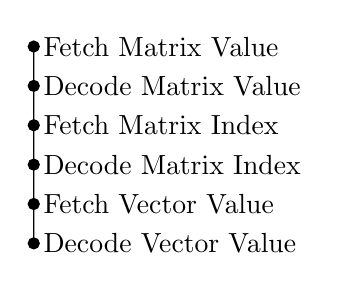
\begin{tikzpicture}
				\filldraw
					(0,2.5) circle (2pt) node[right] {Fetch Matrix Value} --
					(0,2.0) circle (2pt) node[right] {Decode Matrix Value} --
					(0,1.5) circle (2pt) node[right] {Fetch Matrix Index} --
					(0,1.0) circle (2pt) node[right] {Decode Matrix Index} --
					(0,0.5) circle (2pt) node[right] {Fetch Vector Value} --
					(0,0.0) circle (2pt) node[right] {Decode Vector Value};
			\end{tikzpicture}
			\caption{Serial Model.}
		\end{subfigure}
		\begin{subfigure}[t]{0.65\textwidth}
			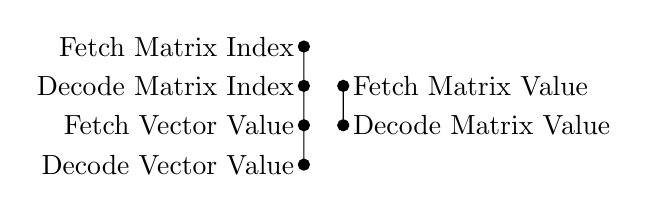
\begin{tikzpicture}
				\filldraw
					(0,2.0) circle (2pt) node[left] {Fetch Matrix Index} --
					(0,1.5) circle (2pt) node[left] {Decode Matrix Index} --
					(0,1.0) circle (2pt) node[left] {Fetch Vector Value} --
					(0,0.5) circle (2pt) node[left] {Decode Vector Value};
				\filldraw
					(0.5,1.5) circle (2pt) node[right] {Fetch Matrix Value} --
					(0.5,1.0) circle (2pt) node[right] {Decode Matrix Value};
			\end{tikzpicture}
			\caption{Parallel Model.}
		\end{subfigure}
	}
	
	\caption[Data dependency graphs for performance models.]{Comparison of the data dependency graphs used by each model, where lower nodes are dependent on higher nodes.}
	\label{fig:models-dataDeps}
\end{figure} %
Note that this model assumes that the compiler and processor can fully parallelize any operations without data dependencies, while, at the absolute minimum, the instructions must be read serially~\cite{Hennessy:1990:ComputerArchitecture}.
Additionally, the model assumes that the bytes of each compressed value is constant, which is not true for most matrix compression and for some vector compression.
Lastly, the model was used with integral values for the bytes, decode times and encode times.
The model then takes the same compression properties as the first model and computes the time to fetch and decode the values and encode the result value over 10 matrix rows with 27 entries per row.
Appendix~\ref{app:decode-model-source} contains source code for this model.

The bounds on outperforming the baseline implementation were hard to determine for the simulation model due to the nature of the model as a sum of maximizations.
However, some boundaries were computed.
Table~\ref{tab:models-singleComp} shows the restrictions when compressing only a single data structure.
\begin{table}
	\begin{tabular}{r|S|S|c}
      & {Matrix Index}  & {Matrix Value} & {Vector}\\
	{Bytes} & {Decode}        & {Decode}       & Encode and Decode \\
	\hline
	1 & 66 & 41 & \(4.75\geq 1.75\cdot\mathrm{decode}+\mathrm{encode}\)\\
	2 & 51 & 14 &\(4.75\geq 1.75\cdot\mathrm{decode}+\mathrm{encode}\)\\
	3 & 66 & 40 &\(2\geq 2\cdot\mathrm{decode}+\mathrm{encode}\)\\
	4 & 0 & 0 &\(0=\mathrm{decode}=\mathrm{encode}\) \\
	5 & {-} & 37 & \(4.75\geq 1.75\cdot\mathrm{decode}+\mathrm{encode}\)\\
	6 & {-} & 9 & Not Possible\\
	7 & {-} & 35 & \(0=\mathrm{decode}=\mathrm{encode}\)\\
	8 & {-} & 0 & \(0=\mathrm{decode}=\mathrm{encode}\)
\end{tabular}

	\caption{Maximum Decode Times in Clocks for Single Structure Compression According to the Simulation Based Model.}
	\label{tab:models-singleComp}
\end{table} %
The matrix index and value columns contain the maximum time to decode a value, in clocks.
The vector column contains equations that restrict the decode and encode time, with values in clocks.
Note that the vector limits are not the only way to compute the restriction.
These compression bounds appear to be significantly related to the frequency at which multiple values are fetched from main memory.

\review{Is there a way to look at combined compression results? Size variables are too strange to be able to do a set of equations}


\section{Test Results}
\label{sec:results}
Tables~\ref{tab:results-vec}, \ref{tab:results-val} and~\ref{tab:results-ind} show the compression results for compressing just the vector values, matrix values and matrix indices respectively.
These tables, and all following tables of test results, contain the rating measured by HPCG, the GFLOP rating with convergance overhead, the number of iterations needed for convergence and, where computed, the compression rate based on the number of cache lines fetched, which may be different then the memory allocated.
Note that some compression strategies had multiple variations that were tested.
Section~\ref{sec:results-vec} contains information on variations used in vector compression.
The compression of just one data structure fails to outperform the baseline implementation; Section~\ref{sec:results-bounds} discusses this further.

%TODO make note of consistancy results (10 runs of baseline had the range of ratings equal to .6128)
%TODO discuss why compiler settings don't have a significant affect on things
	%Consider putting consistancy with compiler settings, both about why these results are good enough
%TODO considering using rating w/out optimization overhead also/instead
%TODO make sure that the results shown don't need to be cut down to be understandable

\begin{table}
	\centering
	\begin{tabular}{l|S[table-format=2.6]|S[table-format=2.6]|r|c}
		            & {HPCG}   & {GFLOPs} &            & Compression \\
		Compression & {Rating} & {Rating} & Iterations & Rate \\
		\hline
		\csvreader[head to column names,separator=semicolon,filter strcmp={\type}{}]{figures/4.Results/Vec.csv}{}{ \tablename & \hpcg & \gflops & \iterations & \rate \\}
		Mixed Precision & & & & \\ %b, x, d, Ad, r, z
		\csvreader[head to column names,separator=semicolon,filter strcmp={\type}{mixed}]{figures/4.Results/Vec.csv}{}{\hspace{3mm}\tablename & \hpcg & \gflops & \iterations & \rate \\}
		ZFP - 1d & & & & \\
			\csvreader[head to column names,separator=semicolon,filter strcmp={\type}{ZFP-1d}]{figures/4.Results/Vec.csv}{}{\hspace{3mm}\tablename & \hpcg & \gflops & \iterations & \rate \\}
		ZFP - 3d & & & & \\
			\csvreader[head to column names,separator=semicolon,filter strcmp={\type}{ZFP-3d}]{figures/4.Results/Vec.csv}{}{\hspace{3mm}\tablename & \hpcg & \gflops & \iterations & \rate \\}
		SZ & & & & \\
		%timings have error setting of 1e-10 abs and 1e-10 rel
		\csvreader[head to column names,separator=semicolon,filter strcmp={\type}{SZ}]{figures/4.Results/Vec.csv}{}{\hspace{3mm}\tablename & \hpcg & \gflops & \iterations & \rate \\}
	\end{tabular}
	\caption{Results of Compressing Vector Values.}
	\label{tab:results-vec}
\end{table}

\begin{table}
	\centering
	\begin{tabular}{l|S[table-format=2.6]|S[table-format=2.6]|r|c}
		            & {HPCG}   & {GFLOPs} &            & Compression \\
		Compression & {Rating} & {Rating} & Iterations & Rate \\
		\hline
		\csvreader[head to column names,filter strcmp={\type}{}]{figures/4.Results/Val.csv}{}{ \tablename & \hpcg & \gflops & \iterations & \rate \\}
		SZ & & & & \\
		\csvreader[head to column names,filter strcmp={\type}{SZ}]{figures/4.Results/Val.csv}{}{\hspace{3mm}\tablename & \hpcg & \gflops & \iterations & \rate \\}
		ZFP & & & & \\
		\csvreader[head to column names,filter strcmp={\type}{ZFP}]{figures/4.Results/Val.csv}{}{\hspace{3mm}\tablename & \hpcg & \gflops & \iterations & \rate \\}
	\end{tabular}
	\caption{Results of Compressing Matrix Values.}
	\label{tab:results-val}
\end{table}
\begin{table}
	\centering
	\begin{tabular}{l|S[table-format=2.6]|S[table-format=2.6]|r|c}
		            & {HPCG}   & {GFLOPs} &            & Compression \\
		Compression & {Rating} & {Rating} & Iterations & Rate \\
		\hline
		\csvreader[head to column names,separator=semicolon,filter strcmp={\type}{}]{figures/4.Results/Ind.csv}{}{ \tablename & \hpcg & \gflops & \iterations & \rate \\}
		Huffman & & & & \\
		\hspace{3mm}No First Index & & & & \\
			\csvreader[head to column names,separator=semicolon,filter strcmp={\type}{huffman-nofirst}]{figures/4.Results/Ind.csv}{}{\hspace{3mm}\tablename & \hpcg & \gflops & \iterations & \rate \\}
		\hspace{3mm}First Index & & & & \\
			%huffman-nofirst;6-bit window;Huffman - No First - 6 bit;10.7666;10.9715;51; \({\sim}1\):9;
			%huffman-nofirst;10-bit window;Huffman - No First - 10 bit;10.8156;11.024;51;\({\sim}3\):10;1
			\csvreader[head to column names,separator=semicolon,filter strcmp={\type}{huffman-first}]{figures/4.Results/Ind.csv}{}{\hspace{6mm}\tablename & \hpcg & \gflops & \iterations & \rate \\}
		%TODO consider adding more Huffman timings (single table, cont alloc)
		Op Code & & & & \\
		\csvreader[head to column names,separator=semicolon,filter strcmp={\type}{opcode}]{figures/4.Results/Ind.csv}{}{\hspace{3mm}\tablename & \hpcg & \gflops & \iterations & \rate \\}
	\end{tabular}
	\caption{Results of compressing matrix indices.}
	\label{tab:results-ind}
\end{table}

Next, combined compression schemes were tried, using SZ and single precision compression for the matrix values and using SZ, gamma and delta compression for the matrix indices.
Table~\ref{tab:results-combined-mat} shows the results of these combined schemes.
The combined scheme with the best performance used SZ compression for both values and indices.
The only other approach that outperformed the baseline implementation used 32 bit compression for the values and gamma compression for the indices.

\begin{table}
	\centering
	\begin{tabular}{l|l|S[table-format=2.6]|S[table-format=2.6]|r}
		\multicolumn{2}{c|}{Compression} & {HPCG} & {GFLOPs} & \\
		Value    &   Index               & {Rating} & {Rating}   & Iterations \\
		\hline
		\multicolumn{2}{c|}{Baseline} & 15.3654 & 15.7394 & 50 \\
		SZ & SZ & 18.9702 & 19.5759 & 50 \\
		SZ & Gamma & 13.661 & 13.9794 & 51 \\
		SZ & Delta & 10.9903 & 11.1961 & 50 \\
		32 bit & SZ & 14.1796 & 14.5156 & 51 \\
		32 bit & Gamma & 17.6676 & 18.1835 & 51 \\
		32 bit & Delta & 12.56 & 12.8181 & 51 \\
	\end{tabular}
	\caption{Results of Combined Matrix Value and Index Compression Schemes.}
	\label{tab:results-combined-mat}
\end{table}
%TODO fill in table

Finally, vector compression was combined with the successful combined matrix compression.
Due to the poor performance of SZ and ZFP vector compression, only the better versions of mixed precision vector compression were used.
Table~\ref{tab:results-combined-vec+mat} shows the results for these compression strategies.
The first column indicates which vectors were stored in 32bit; the rest of the columns correspond to their counter parts in Table~\ref{tab:results-combined-mat}.
Note that vector compression improved the performance of the SZ compressed matrices, but reduced the performance of the gamma compressed matrices.
So, the best implementation for the test problem uses mixed precision vectors with \(\vec{b}, \vec{x}\) and \(\mat{A}\vec{d}\) stored in single precision, and sz compressed matrix values and indices.

\begin{table}
	\centering
	\begin{tabular}{l|l|l|S|r}
		\multicolumn{3}{c|}{Compression} & & \\
		32 bit   &       &       &        &            \\
		Vectors & Value & Index & GFLOPs & Iterations \\
		\hline
		\multicolumn{3}{c|}{Baseline} & 15.3654 & 50 \\
		None & SZ & SZ & 18.9702 & 50 \\
		\(\vec{b}, \vec{x}\) & SZ & SZ & 23.967 & 50 \\
		\(\vec{b}, \vec{x}, \mat{A}\vec{d}\) & SZ & SZ & 27.5974 & 50 \\
		None & 32 bit & Gamma & 17.6676 & 51 \\
%I don't think these need to be shown
%		\(\vec{b}\) & 32 bit & Gamma & 16.4514 & 50 \\
%		\(\vec{x}\) & 32 bit & Gamma & 16.6688 & 50 \\
		\(\vec{b}, \vec{x}\) & 32 bit & Gamma & 16.6048 & 50 \\
		\(\vec{b}, \vec{x}, \mat{A}\vec{d}\) & 32 bit & Gamma & 16.5665 & 50 \\
	\end{tabular}
	\caption{Results of Combined Vector, Matrix Value and Matrix Index Compression Schemes.}
	\label{tab:results-combined-vec+mat}
\end{table}
%TODO fill in table

\subsection{Performance Improvement Bounds}
\label{sec:results-bounds}
Note that Table~\ref{tab:results-val} shows 1 bit compression under performing the baseline implementation, even though it has a significant compression rate.
This demonstrates that compressing the matrix values alone in unable to improve performance.
For the vector values, note that the single precision implementation has a 2.3 times increase in iterations to convergence over the baseline implementation and that the GFLOPs rating of the single precision implementation is reduced by a factor of approximately 2.19 from the baseline implementation.
This hints that, even without increasing the number of Conjugate Gradient iterations, compressing the vectors requires a compression rate better than 1:2 to provide much of an improvement in performance.
This analysis is supported by the fact that none of the compression strategies tried that only compressed a single strategy where able to out perform the baseline implementation.

\subsection{Vector Compression}
\label{sec:results-vec}
As shown in Table~\ref{tab:results-vec}, vector compression was not successfully used to improve performance.
Section~\ref{sec:results-bounds} discusses why performance improvement is likely limited.
However, vector compression is able to make improvements when combined with other compressions, as shown in Table~\ref{tab:results-combined-vec+mat}.

ZFP had poor performance when compressing vector information.
The high level array API was used to provide the necessary random access.
Note that 1 dimensional ZFP compression has a 16 bit granularity, and 3 dimensional ZFP compression has a 1 bit granularity~\cite{Lindstrom:2014:zfp}.
These granularity restrictions and the resulting iterations needed were used to select the tested compression rates.

SZ compression has two main configurable settings, the number of values in each block and the error bound.
There were two measures of error that were considered, absolute error and pointwise relative error.
The performance was tested with both a single error being bounded and both errors being bounded.
Absolute error is the absolute value of the difference between predicted and actual.
The pointwise relative error is the absolute error divided by the actual value.
Table~\ref{tab:results-vec} contains results for various block sizes with both an absolute error bound of \(10^{-10}\) and a pointwise relative error bound of \(10^{-10}\).
Table~\ref{tab:results-vec-SZ} contains an comparison of various error bounds for a block size of 8 values per block.
%TODO get timings with another block size (12 val blocks?)
Note that an absolute bound of \(10^{-2}\) was unable to converge within 500 iterations.
%TODO is this note useful?

\begin{table}
	\centering
	\begin{tabular}{l|S|r}
		Error Bound & {GFLOP Rating} & Iterations \\
		\hline
		\(10^{-2}\) relative & 3.66859 & 69 \\
		\(10^{-6}\) relative & 5.7806 & 57 \\
		\(10^{-10}\) relative & 5.78711 & 57 \\
		\(10^{-14}\) relative & 5.81357 & 57 \\
		\(10^{-18}\) relative & 5.73277 & 57 \\
		\(10^{-2}\) absolute & {Unknown} & \(\geq 500\) \\
		\(10^{-6}\) absolute & 4.51827 & 57 \\
		\(10^{-10}\) absolute & 5.14058 & 57\\
		\(10^{-14}\) absolute & 5.64338 & 57 \\
		\(10^{-18}\) absolute & 5.81642 & 57 \\
		\(10^{-2}\) absolute and \(10^{-10}\) relative & 5.75538 & 57 \\
		\(10^{-10}\) absolute and \(10^{-2}\) relative & 5.22592 & 57 \\
		\(10^{-10}\) absolute and \(10^{-10}\) relative & 5.82527 & 57 \\
%TODO figure out if "or" tests should be used
%		\(10^{-2}\) absolute or \(10^{-10}\) relative & 5.77713 & 57 \\
%		\(10^{-10}\) absolute or \(10^{-2}\) relative & 5.16793 & 57 \\
%		\(10^{-10}\) absolute or \(10^{-10}\) relative & 5.80555 & 57 \\
	\end{tabular}
	\caption{Results of Compressing Vector Values with SZ Compression using Various Error Bounds.}
	\label{tab:results-vec-SZ}
\end{table}

\subsection{Testing Environment}
The timings presented were obtained when using a problem size of \(96^3\) matrix rows.
The cluster used for timings had a 20 core, 2.2 GHz Intel Xeon E5-2698 v4 head node and an additional five 8 core, 1.7GHz Intel Xeon E5-2605 nodes.
One process was created for each core, with a single OMP thread per process.

The code was implemented using version 3.0.0 of the HPCG benchmark~\cite{Dongarra:2015:HPCG}.
The code was compiled with the OpenMPI cxx wrapper using GCC version 4.8.5.
OpenMPI 3.2 was used for the compiler wrapper and MPI runtime.
The O3 and fopenmp flags were used for compilation, in addition to a selection of warning flags and the std flag as necessary.

\section{Conclusions}
Data compression was able to successfully increase the performance of the sparse linear solver in HPCG~\cite{Dongarra:2015:HPCG}.
The best performance increase came from using SZ compression on the matrix indices and values and using single precision values for select vectors with an increase in the effective GFLOPs of about 84\%.
However, there are only a few compression strategies that outperform the baseline.

\review{Should this analysis of compression effectiveness be located somewhere else?  With the results?}
When considering more general matrices, note that the effectiveness of SZ compression is highly dependent on local relationships between compressed values.
So, SZ based compression strategies will likely lose performance on many other matrices.
However, note that the performance of single precision ``compression'' is unaffected by the values being compressed and that the effectiveness of gamma compression is proportional to the number of significant bits.
Thus, using 32bit matrix values and gamma compressed matrix indices will likely perform more consistently than the SZ based compression approach and may perform better on some matrices.

\subsection{Future Work}
\review{this order/organization of these paragraphs}
The two general directions this work can be extended are applying compression to different setups and changing the compression used.
The first direction extends this idea of this project to more general situations, including different matrices or solvers.
The second direction would provide either better compression for this problem, or hint that the effective compression methods can't be significantly outperformed.
In addition to extensions to this project, work could be done using this idea of compression in real work software packages.

Note that the stencil matrix used by HPCG is very consistent and has a large amount of repetition; this makes it easy to compress.
So, experimenting with other matrices could provide a more general idea of the performance.
The SuiteSparse Matrix Collection provides linear systems that could be used for such a project~\cite{Davis:2011:FloridaMatrixCollection}.
However, note that the HPCG implementation makes some assumptions about the matrix in the problem setup, so some of the setup sections would need to be rewritten~\cite{Dongarra:2015:HPCG}.

Another aspect that could be further experimented with is the solver used.
Other solvers and preconditioner likely have different data access patterns than the solver used in HPCG.
These differences may change the available compression strategies, have different precision requirements or have different ratios of memory fetches to arithmetic.
So, different solvers may have better optimal compression strategies.
Additionally, GPU accelerated solvers may differ due to the differences in GPU execution and performance.

The last area this work could be extended would be trying different compression methods or variants of the compression methods used in this project.
On such topic would be looking at using different error tolerances for different vectors, like what is done with single precision compression.
Another possible variation would be to compress additional data structures, such as the matrix diagonals.
Finally, totally new compression strategies could be used.



\bibliographystyle{plain}
\bibliography{bibliograph}

\appendix

\section{Performance Model Source Code}
\label{app:decode-model-source}
Below is the implementation of the simulation based performance model.
The model was implemented in Common Lisp and used with Steel Bank Common Lisp version 1.4.0.

%TODO out of date
\begin{lstlisting}[language=Lisp,
					showstringspaces=false,
					numbers=left,
					numberstyle=\tiny]
;;; Global Variables

; Cluster properties
(defparameter *l1-time* 5)
(defparameter *l2-time* 12)
(defparameter *main-mem-time* 1656/10)

; Model parameters
(defparameter *rows-to-check* 128)

; Default compression settings
(defparameter *bytes-per-mat-ind* 4)
(defparameter *bytes-per-mat-val* 8)
(defparameter *bytes-per-vect* 8)
(defparameter *inds-decode-time* 0)
(defparameter *vals-decode-time* 0)
(defparameter *vect-decode-time* 0)
(defparameter *vect-encode-time* 0)


;;; Model Implementation

(defmethod fetch ((obj (eql :mat-inds)) (i integer))
  "Computes the cost of fetching the ith matrix index"
  (if (/= (floor (* (1- i) *bytes-per-mat-ind*) 64)
          (floor (* i *bytes-per-mat-ind*) 64))
    *main-mem-time*
    *l1-time*))

(defmethod fetch ((obj (eql :mat-vals)) (i integer))
  "Computes the cost of fetching the ith matrix value"
  (if (/= (floor (* (1- i) *bytes-per-mat-val*) 64)
          (floor (* i *bytes-per-mat-val*) 64))
    *main-mem-time*
    *l1-time*))

(defmethod fetch ((obj (eql :vect)) (i integer))
  "Computes the code of fetching the ith vector value"
  (cond
    ; 2/3rds of values were used by the previous index
    ((/= (mod i 3) 2) *l1-time*)
    ; 2/9ths of values were used by y-1
    ((< (/ i 3) 6) *l2-time*)
    ; 1/9th of values are being used for the first time
    (t (if (/= (floor (* (1- (/ i 27)) *bytes-per-vect*)
                      64)
               (floor (* (/ i 27) *bytes-per-vect*)
                      64))
         *main-mem-time*
         *l1-time*))))


(defun 1-row ()
  "Computings the average cost to load a row.
   *rows-to-check* provides the number of rows to use"
  (+ (/ (loop
          :for i :from 0 :below (* *rows-to-check* 27)
          :for inds-fetch-time = (fetch :mat-inds i)
          :for vals-fetch-time = (fetch :mat-vals i)
          :for vect-fetch-time = (fetch :vect i)
          :for total-vals-time = (+ vals-fetch-time
                                    *vals-decode-time*)
          :for total-vect-time = (+ inds-fetch-time
                                    *inds-decode-time*
                                    vect-fetch-time
                                    *vect-decode-time*)
          :summing (min total-vals-time total-vect-time))
        *rows-to-check*)
     *vect-encode-time*))


(defun 1-row-with-props (ind-size val-size vect-size
                         ind-decode val-decode
                         vect-decode vect-encode)
  "Like 1-row, but sets the compression properties"
  (let ((*bytes-per-mat-ind* ind-size)
        (*bytes-per-mat-val* val-size)
        (*bytes-per-vect* vect-size)
        (*inds-decode-time* ind-decode)
        (*vals-decode-time* val-decode)
        (*vect-decode-time* vect-decode)
        (*vect-encode-time* vect-encode))
    (1-row)))


\end{lstlisting}
 

\end{document}